\documentclass[a4paper,12pt]{article}
\usepackage{czech}
\usepackage[utf8]{inputenc}
\usepackage{a4wide}
\usepackage[dvipdfm]{graphicx}
\usepackage{graphics}
\usepackage{indentfirst}
\usepackage{fancyhdr}
\usepackage{setspace}
\usepackage{amsmath}
\usepackage{amssymb}
\usepackage{epsfig}
\usepackage{multirow}

%%\usepackage{nopageno}
%%\usepackage{txfonts}
\usepackage[usenames]{color}

\begin{document}
\section{Úkol}
\noindent
\begin{enumerate}
    \item   Změřte statickou charakteristiku termistoru pro proudy do 25 mA a graficky ji znázorněte.
    \item   Změřte teplotní závislost odporu termistoru v teplotním intervalu přibližně 180 až 380 K.
    \item   Graficky znázorněte závislost logaritmu odporu $R$ termistoru na $1/T$ a vyhodnoťte velikost 
    materiálových veličin $R_\infty$ a $B$, aktivační energie $U$ a teplotního součinitele odporu při pokojové teplotě.
    \item   Stanovte teplotu termistoru v maximu charakteristiky, případně v některých dalších bodech a tepelný odpor $K$. 
\end{enumerate}

\section{Teorie}

\subsection{Termistor}
Termistor je polovodičová součástka, jejíž odpor je závislý na teplotě. Tato závislost je vajádřena vztahem
\begin{eqnarray}
    R=R_\infty \exp(B/T),
    \label{R}
\end{eqnarray}
kde $R_\infty$ je dán materriálem, ze kterého je termistor vyroben a $B$ udává jeho citlivost na teplotu.

Pro $B$ kovalentních polovodičů platí vztah
\begin{eqnarray}
    B=\frac{\Delta U}{2k},
    \label{B}
\end{eqnarray}
kde $k$ je Boltzmannova konstanta a $\Delta U$ ionizační energie příměsi.

\subsection{Teplotní součinitel odporu}
Teplotní součinitel odporu se značí $\alpha$ a je definovát vztahem
\begin{eqnarray}
    \alpha=\frac{1}{R(T)}\frac{\mbox{d}R(T)}{\mbox{d}T}.
\end{eqnarray}

Pro termistor můžeme za $R$ dosadit z rovnice \ref{R} a získáme
\begin{eqnarray}
    \alpha=-\frac{B}{T^2}.
    \label{alpha}
\end{eqnarray}

\subsection{Aktivační eneergie}
Za předpokladu, že známe dva odpory $R_1$ a $R_2$ pro různé teploty $T_1$ a $T_2$, můžeme určit $B$ ze vztahu
\begin{eqnarray}
    B=\frac{2.3\cdot\ln(R_1/R_2)}{1/T_1-1/T_2}.
\end{eqnarray}

\subsection{Určení $R_\infty$}
Pokud zlogaritmujeme rovnici \ref{R}, získáme
\begin{eqnarray}
    \ln R=\ln R_\infty+0.434B/T.
\end{eqnarray}
Pak již stačí jen $1/T \to 0$ a získáme hodnotu $R_\infty$.

\subsection{Statická charakteristika termisoru}
Jedná se VA charakteristiku termistoru pro určitou teplotu. Jak je vidět z obrázku \ref{VA}, Ohmův zákon zorhodně neplatí. 
Je to dáno tím, že průchodem proudu se termistor zahřívá, a tím se mění i jeho odpor. Pro napětí na termistoru je v \cite{text} 
odvozen výraz
\begin{eqnarray}
U=\sqrt{\frac{R_\infty\cdot(T-T_0)\exp(B/T)}{K}},
\end{eqnarray}
kde $K$ je tepelný odpor rezistoru. Pro maximum dále platí
\begin{eqnarray}
T_m=\frac{1}{2}(B-\sqrt{B(B-4T)}).
\end{eqnarray}

\subsection{Stanovení tepelněho odporu}
Za předpokladu, že známe průběh odporu termistoru v závislosti na napětí, můžeme stanovit jeho teplotu pro určitý proud a napětí (Ohmův zákon). 
Z toho pak můžeme určit tepelný odpor dle vztahu
\begin{eqnarray}
K=\frac{T_x-T_0}{U_xI_x},
\end{eqnarray}
kde indexy $m$ označují veličiny pro daný bod charakteristiky a $T_0$ je teplota prostředí.

\subsection{Platinový odporový teploměr}
Odpor tohoto teploměru se mění lineárně se změnou teploty. Díky tomu můžeme určit teplotu dle vztahu
\begin{eqnarray}
T=\frac{R_t-R_0}{\alpha R_0},
\end{eqnarray}
kde pro náš teploměr platí $R_0 = 100 \Omega$ a $\alpha = 3.85\cdot10^{-3}$ K$^{-1}$.

\subsection{Schéma zapojení}
Celé měření probíhá v zapojení dle obrázku \ref{sch1}. V našem případě jsme pouze vyjmuli potenciometr a napětí regulujeme na zdroji.

\subsection{Chyby}
Veškeré chyby měření jsou určené nepřesností měřících přístrojů. Použil jsem pouze dva multimetry typu MXD-4660 A, jejiž nepřesnosti 
jsou uvedeny pro jednotlivé veličiny a rozsahy v tabulce \ref{TChyby}. Pokud není v tabulce uveden rozsah, znamená to, že daná nepřesnost platí pro všechny 
použité rozsahy. Tyto přístroje zobrazovali 5 cifer.

\begin{table}
\begin{center}
\begin{tabular}{|c|c|c|}
\hline
DC V&   &   $\pm 0.5 \%$ + 3d \\ \hline
DC A&   &   $\pm 0.3 \%$ + 3d \\ \hline
\multirow{4}{*}{$\Omega$}&   200 $\Omega$&   $\pm 0.2 \%$ + 5d \\ \cline{2-3}
&   2k$\Omega$& \multirow{3}{*}{$\pm 0.15 \%$ + 3d} \\
&   \vdots&  \\ 
&   20M$\Omega$& \\ \hline
\end{tabular}
\end{center}
\caption{Nepřesnosti multimetru MXD-4660 A}
\label{TChyby}
\end{table}

\begin{figure}
\begin{center}
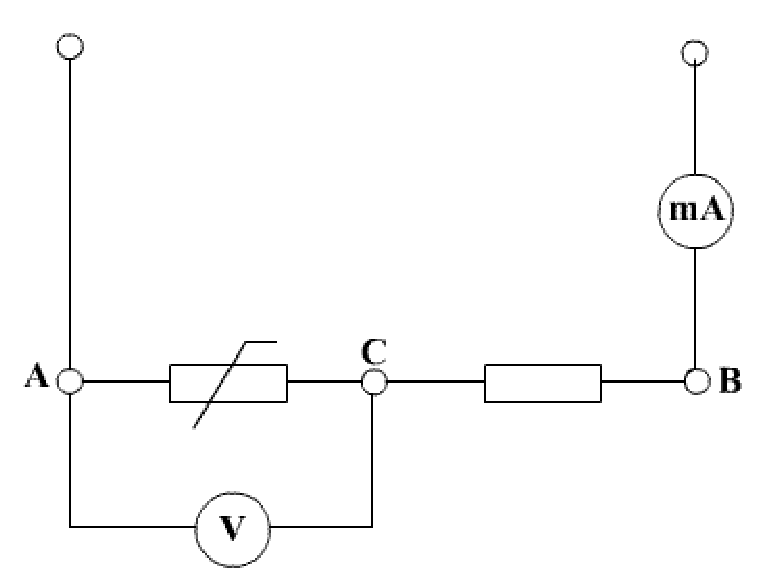
\includegraphics[width=4in]{sch1.eps}
\end{center}
\caption{Schéma zapojení při měření.}
\label{sch1}
\end{figure}

\begin{figure}
\begin{center}
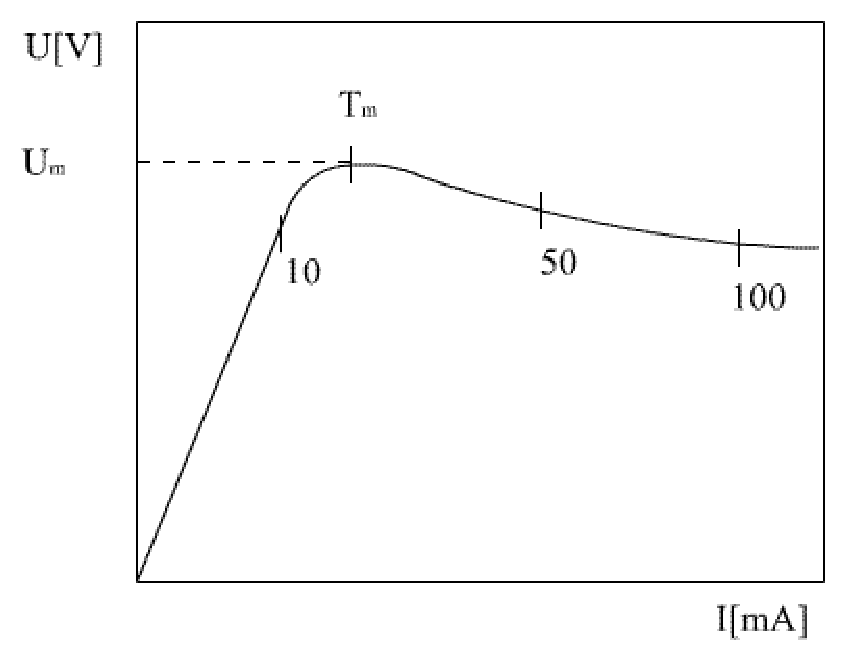
\includegraphics[width=4in]{VA.eps}
\end{center}
\caption{VA charakteristika termistoru z konstantní teploty okolí.}
\label{VA}
\end{figure}

\section{Výsledky měření}

\subsection{Statická charakteristika termočlánku}
V zapojení popsaném v teorii jsem měřil velikost proudu v obvodu v závislosti na vstupním napětí. 
Hodnoty z multimetrů jsem zaznamenával pomocí programu Termistor do počítače. Dále jsem vyhodnotil 
chybu měření a výsledkem je tabulka \ref{TVA}. Její grafické znázornění je obrázek \ref{g1}.

\begin{table}
$$
\begin{array}{|c|c|}
\hline
I/\mbox{mA}& U/\mbox{V} \\ \hline
0.109\pm 0.002&0.0544\pm 0.0005\\ \hline
0.202\pm 0.004&0.1006\pm 0.0006\\ \hline
0.302\pm 0.005&0.1505\pm 0.0008\\ \hline
0.407\pm 0.005&0.2021\pm 0.0009\\ \hline
0.503\pm 0.006&0.249\pm 0.001\\ \hline
0.605\pm 0.006&0.298\pm 0.001\\ \hline
0.705\pm 0.007&0.346\pm 0.004\\ \hline
0.804\pm 0.007&0.392\pm 0.004\\ \hline
0.909\pm 0.008&0.440\pm 0.004\\ \hline
1.013\pm 0.008&0.487\pm 0.004\\ \hline
2.18\pm 0.04&0.929\pm 0.006\\ \hline
3.03\pm 0.05&1.153\pm 0.006\\ \hline
4.00\pm 0.05&1.331\pm 0.007\\ \hline
5.08\pm 0.06&1.463\pm 0.007\\ \hline
6.15\pm 0.06&1.544\pm 0.008\\ \hline
7.03\pm 0.07&1.587\pm 0.008\\ \hline
8.14\pm 0.07&1.622\pm 0.008\\ \hline
8.60\pm 0.07&1.631\pm 0.008\\ \hline
9.05\pm 0.08&1.640\pm 0.008\\ \hline
9.48\pm 0.08&1.644\pm 0.008\\ \hline
10.05\pm 0.08&1.651\pm 0.008\\ \hline
10.46\pm 0.08&1.652\pm 0.008\\ \hline
11.10\pm 0.09&1.657\pm 0.008\\ \hline
11.60\pm 0.09&1.657\pm 0.008\\ \hline
12.09\pm 0.09&1.657\pm 0.008\\ \hline
12.48\pm 0.09&1.656\pm 0.008\\ \hline
13.18\pm 0.10&1.655\pm 0.008\\ \hline
14.1\pm 0.1&1.651\pm 0.008\\ \hline
15.4\pm 0.1&1.645\pm 0.008\\ \hline
16.0\pm 0.1&1.640\pm 0.008\\ \hline
17.0\pm 0.1&1.634\pm 0.008\\ \hline
19.2\pm 0.1&1.617\pm 0.008\\ \hline
20.0\pm 0.4&1.610\pm 0.008\\ \hline
21.0\pm 0.4&1.603\pm 0.008\\ \hline
22.1\pm 0.4&1.595\pm 0.008\\ \hline
23.1\pm 0.4&1.589\pm 0.008\\ \hline
24.0\pm 0.4&1.582\pm 0.008\\ \hline
25.0\pm 0.4&1.576\pm 0.008\\ \hline
\end{array}
$$
\caption{Tabulka VA charakteristiky termočlánku}
\label{TVA}
\end{table}

\begin{figure}
\scalebox{0.7}{
% GNUPLOT: LaTeX picture with Postscript
\begingroup
  \makeatletter
  \providecommand\color[2][]{%
    \GenericError{(gnuplot) \space\space\space\@spaces}{%
      Package color not loaded in conjunction with
      terminal option `colourtext'%
    }{See the gnuplot documentation for explanation.%
    }{Either use 'blacktext' in gnuplot or load the package
      color.sty in LaTeX.}%
    \renewcommand\color[2][]{}%
  }%
  \providecommand\includegraphics[2][]{%
    \GenericError{(gnuplot) \space\space\space\@spaces}{%
      Package graphicx or graphics not loaded%
    }{See the gnuplot documentation for explanation.%
    }{The gnuplot epslatex terminal needs graphicx.sty or graphics.sty.}%
    \renewcommand\includegraphics[2][]{}%
  }%
  \providecommand\rotatebox[2]{#2}%
  \@ifundefined{ifGPcolor}{%
    \newif\ifGPcolor
    \GPcolorfalse
  }{}%
  \@ifundefined{ifGPblacktext}{%
    \newif\ifGPblacktext
    \GPblacktexttrue
  }{}%
  % define a \g@addto@macro without @ in the name:
  \let\gplgaddtomacro\g@addto@macro
  % define empty templates for all commands taking text:
  \gdef\gplbacktext{}%
  \gdef\gplfronttext{}%
  \makeatother
  \ifGPblacktext
    % no textcolor at all
    \def\colorrgb#1{}%
    \def\colorgray#1{}%
  \else
    % gray or color?
    \ifGPcolor
      \def\colorrgb#1{\color[rgb]{#1}}%
      \def\colorgray#1{\color[gray]{#1}}%
      \expandafter\def\csname LTw\endcsname{\color{white}}%
      \expandafter\def\csname LTb\endcsname{\color{black}}%
      \expandafter\def\csname LTa\endcsname{\color{black}}%
      \expandafter\def\csname LT0\endcsname{\color[rgb]{1,0,0}}%
      \expandafter\def\csname LT1\endcsname{\color[rgb]{0,1,0}}%
      \expandafter\def\csname LT2\endcsname{\color[rgb]{0,0,1}}%
      \expandafter\def\csname LT3\endcsname{\color[rgb]{1,0,1}}%
      \expandafter\def\csname LT4\endcsname{\color[rgb]{0,1,1}}%
      \expandafter\def\csname LT5\endcsname{\color[rgb]{1,1,0}}%
      \expandafter\def\csname LT6\endcsname{\color[rgb]{0,0,0}}%
      \expandafter\def\csname LT7\endcsname{\color[rgb]{1,0.3,0}}%
      \expandafter\def\csname LT8\endcsname{\color[rgb]{0.5,0.5,0.5}}%
    \else
      % gray
      \def\colorrgb#1{\color{black}}%
      \def\colorgray#1{\color[gray]{#1}}%
      \expandafter\def\csname LTw\endcsname{\color{white}}%
      \expandafter\def\csname LTb\endcsname{\color{black}}%
      \expandafter\def\csname LTa\endcsname{\color{black}}%
      \expandafter\def\csname LT0\endcsname{\color{black}}%
      \expandafter\def\csname LT1\endcsname{\color{black}}%
      \expandafter\def\csname LT2\endcsname{\color{black}}%
      \expandafter\def\csname LT3\endcsname{\color{black}}%
      \expandafter\def\csname LT4\endcsname{\color{black}}%
      \expandafter\def\csname LT5\endcsname{\color{black}}%
      \expandafter\def\csname LT6\endcsname{\color{black}}%
      \expandafter\def\csname LT7\endcsname{\color{black}}%
      \expandafter\def\csname LT8\endcsname{\color{black}}%
    \fi
  \fi
  \setlength{\unitlength}{0.0500bp}%
  \begin{picture}(11904.00,8502.00)%
    \gplgaddtomacro\gplbacktext{%
      \csname LTb\endcsname%
      \put(1078,704){\makebox(0,0)[r]{\strut{} 0}}%
      \put(1078,2488){\makebox(0,0)[r]{\strut{} 0,5}}%
      \put(1078,4273){\makebox(0,0)[r]{\strut{} 1}}%
      \put(1078,6057){\makebox(0,0)[r]{\strut{} 1,5}}%
      \put(1078,7841){\makebox(0,0)[r]{\strut{} 2}}%
      \put(1210,484){\makebox(0,0){\strut{} 0}}%
      \put(3203,484){\makebox(0,0){\strut{} 5}}%
      \put(5196,484){\makebox(0,0){\strut{} 10}}%
      \put(7189,484){\makebox(0,0){\strut{} 15}}%
      \put(9182,484){\makebox(0,0){\strut{} 20}}%
      \put(11174,484){\makebox(0,0){\strut{} 25}}%
      \put(308,4272){\rotatebox{-270}{\makebox(0,0){\strut{}\rotatebox{-90}{$\frac{U}{\mathrm{V}}$}}}}%
      \put(6391,154){\makebox(0,0){\strut{}$\frac{I}{\mathrm{mA}}$}}%
      \put(6391,8171){\makebox(0,0){\strut{}Graf 1: Z\'avislost nap\v{e}t\'i na proudu}}%
    }%
    \gplgaddtomacro\gplfronttext{%
      \csname LTb\endcsname%
      \put(10586,1482){\makebox(0,0)[r]{\strut{}$U(I)$}}%
      \csname LTb\endcsname%
      \put(10586,1196){\makebox(0,0)[r]{\strut{}$U(I)$}}%
      \csname LTb\endcsname%
      \put(10586,910){\makebox(0,0)[r]{\strut{}$T_m$}}%
    }%
    \gplbacktext
    \put(0,0){\includegraphics{graf1}}%
    \gplfronttext
  \end{picture}%
\endgroup

}
\label{g1}
\end{figure}

\subsection{TEplotní závislost odporu termistoru}
Za pokojové teploty, která byla dle teploměru v místnosti $T=24.4 ^o$C byl odpor termistoru
\begin{eqnarray}
R_t=0.4602 \mbox{k}\Omega
\end{eqnarray}
a platinového teploměru
\begin{eqnarray}
R_p=109.27 \Omega,
\end{eqnarray}
což odpovídá teplotě 24 $^o$C.

Dále byl termistor zchlazen tekutým dusíkem a pomocí počítače jsem zaznamenával odpory 
na platinovém teploměru a termistoru. V vypočtenou teplotou jsou daata shrnuty v tabulce \ref{TTR}.

\begin{table}
$$
\begin{array}{|c||c|c|}
\hline
R_p/\Omega& T/\mbox{K}& R_t/\mbox{k}\Omega\\ \hline
65.0\pm 0.1&-0.9\pm-0.1&116.4\pm 0.5\\ \hline
67.0\pm 0.4&-0.9\pm-0.3&80.7\pm 0.4\\ \hline
69.0\pm 0.4&-0.8\pm-0.3&57.3\pm 0.1\\ \hline
71.0\pm 0.4&-0.8\pm-0.3&41.53\pm 0.09\\ \hline
73.0\pm 0.4&-0.7\pm-0.3&30.59\pm 0.08\\ \hline
75.0\pm 0.4&-0.6\pm-0.3&22.71\pm 0.06\\ \hline
77.0\pm 0.4&-0.6\pm-0.2&16.76\pm 0.06\\ \hline
79.0\pm 0.4&-0.5\pm-0.2&12.70\pm 0.05\\ \hline
81.0\pm 0.4&-0.5\pm-0.2&9.74\pm 0.04\\ \hline
83.0\pm 0.4&-0.4\pm-0.2&7.54\pm 0.04\\ \hline
85.0\pm 0.4&-0.4\pm-0.2&5.84\pm 0.01\\ \hline
87.0\pm 0.4&-0.3\pm-0.1&4.581\pm 0.010\\ \hline
89.0\pm 0.4&-0.3\pm-0.1&3.621\pm 0.008\\ \hline
91.0\pm 0.4&-0.2\pm-0.1&2.783\pm 0.007\\ \hline
93.0\pm 0.4&-0.2\pm-0.1&2.211\pm 0.006\\ \hline
95.0\pm 0.4&-0.1\pm-0.1&1.731\pm 0.006\\ \hline
97.0\pm 0.4&-0.1\pm-0.0&1.423\pm 0.005\\ \hline
99.0\pm 0.4&-0.0\pm-0.0&1.170\pm 0.005\\ \hline
101.0\pm 0.5&0.0\pm0.0&0.970\pm 0.004\\ \hline
103.0\pm 0.5&0.1\pm0.0&0.790\pm 0.004\\ \hline
105.0\pm 0.5&0.1\pm0.1&0.658\pm 0.001\\ \hline
107.0\pm 0.5&0.2\pm0.1&0.556\pm 0.001\\ \hline
109.0\pm 0.5&0.2\pm0.1&0.471\pm 0.001\\ \hline
111.0\pm 0.5&0.3\pm0.1&0.4021\pm 0.0009\\ \hline
113.0\pm 0.5&0.3\pm0.2&0.3449\pm 0.0008\\ \hline
115.0\pm 0.5&0.4\pm0.2&0.2973\pm 0.0007\\ \hline
117.0\pm 0.5&0.4\pm0.2&0.2573\pm 0.0007\\ \hline
119.0\pm 0.5&0.5\pm0.2&0.2233\pm 0.0006\\ \hline
121.1\pm 0.5&0.5\pm0.3&0.1934\pm 0.0009\\ \hline
123.0\pm 0.5&0.6\pm0.3&0.1713\pm 0.0008\\ \hline
125.0\pm 0.5&0.6\pm0.3&0.1511\pm 0.0008\\ \hline
127.0\pm 0.5&0.7\pm0.3&0.1338\pm 0.0008\\ \hline
129.0\pm 0.5&0.8\pm0.4&0.1190\pm 0.0007\\ \hline
130.0\pm 0.5&0.8\pm0.4&0.1124\pm 0.0007\\ \hline
\end{array}
$$
\caption{Závislost odporu termistoru na teplotě.}
\label{TTR}
\end{table}

\subsection{Závislost log $R$ na 1/$T$}
Za pomoci programu gnuplot jsem nafitoval naměřeným hodnotám přímku, která je na obrázku \ref{g2}. Fit dává hodnoty
\begin{eqnarray}
B=(3140\pm 10) \mbox{K},\\
R_\infty=(0.0138\pm 0.0005) \mbox{k}\Omega.
\end{eqnarray}
Z rovnice \ref{B} získáme aktivační energii, která je rovna 
\begin{eqnarray}
\Delta U=(8670\pm30)\cdot10^{-23} \mbox{J}
\end{eqnarray}
a z rovnice \ref{alpha} vypočteme teplotní součinitel odporu pro teplotu 24.4 $^o$C, který je
\begin{eqnarray}
\alpha=(-0.0355\pm0.0003)\mbox{K}^{-1}
\end{eqnarray}

\subsection{Teplotní maximum termistoru}
Na obrázku \ref{g1} je vyznačeno maximum charakteristiky. Maximum charakteristiky odpovídá teplotě
\begin{eqnarray}
T_m=284.6\pm0.2 \mbox{K}.
\end{eqnarray}
Tepelný odpor termistoru jsem 
určil fitem závislosti výkonu na odporu na obrázku \ref{g3}, který dal hodnotu
\begin{eqnarray}
K=(2050\pm10)\mbox{KW}^{-1}
\end{eqnarray}

\begin{figure}
\scalebox{0.7}{
% GNUPLOT: LaTeX picture with Postscript
\begingroup
  \makeatletter
  \providecommand\color[2][]{%
    \GenericError{(gnuplot) \space\space\space\@spaces}{%
      Package color not loaded in conjunction with
      terminal option `colourtext'%
    }{See the gnuplot documentation for explanation.%
    }{Either use 'blacktext' in gnuplot or load the package
      color.sty in LaTeX.}%
    \renewcommand\color[2][]{}%
  }%
  \providecommand\includegraphics[2][]{%
    \GenericError{(gnuplot) \space\space\space\@spaces}{%
      Package graphicx or graphics not loaded%
    }{See the gnuplot documentation for explanation.%
    }{The gnuplot epslatex terminal needs graphicx.sty or graphics.sty.}%
    \renewcommand\includegraphics[2][]{}%
  }%
  \providecommand\rotatebox[2]{#2}%
  \@ifundefined{ifGPcolor}{%
    \newif\ifGPcolor
    \GPcolorfalse
  }{}%
  \@ifundefined{ifGPblacktext}{%
    \newif\ifGPblacktext
    \GPblacktexttrue
  }{}%
  % define a \g@addto@macro without @ in the name:
  \let\gplgaddtomacro\g@addto@macro
  % define empty templates for all commands taking text:
  \gdef\gplbacktext{}%
  \gdef\gplfronttext{}%
  \makeatother
  \ifGPblacktext
    % no textcolor at all
    \def\colorrgb#1{}%
    \def\colorgray#1{}%
  \else
    % gray or color?
    \ifGPcolor
      \def\colorrgb#1{\color[rgb]{#1}}%
      \def\colorgray#1{\color[gray]{#1}}%
      \expandafter\def\csname LTw\endcsname{\color{white}}%
      \expandafter\def\csname LTb\endcsname{\color{black}}%
      \expandafter\def\csname LTa\endcsname{\color{black}}%
      \expandafter\def\csname LT0\endcsname{\color[rgb]{1,0,0}}%
      \expandafter\def\csname LT1\endcsname{\color[rgb]{0,1,0}}%
      \expandafter\def\csname LT2\endcsname{\color[rgb]{0,0,1}}%
      \expandafter\def\csname LT3\endcsname{\color[rgb]{1,0,1}}%
      \expandafter\def\csname LT4\endcsname{\color[rgb]{0,1,1}}%
      \expandafter\def\csname LT5\endcsname{\color[rgb]{1,1,0}}%
      \expandafter\def\csname LT6\endcsname{\color[rgb]{0,0,0}}%
      \expandafter\def\csname LT7\endcsname{\color[rgb]{1,0.3,0}}%
      \expandafter\def\csname LT8\endcsname{\color[rgb]{0.5,0.5,0.5}}%
    \else
      % gray
      \def\colorrgb#1{\color{black}}%
      \def\colorgray#1{\color[gray]{#1}}%
      \expandafter\def\csname LTw\endcsname{\color{white}}%
      \expandafter\def\csname LTb\endcsname{\color{black}}%
      \expandafter\def\csname LTa\endcsname{\color{black}}%
      \expandafter\def\csname LT0\endcsname{\color{black}}%
      \expandafter\def\csname LT1\endcsname{\color{black}}%
      \expandafter\def\csname LT2\endcsname{\color{black}}%
      \expandafter\def\csname LT3\endcsname{\color{black}}%
      \expandafter\def\csname LT4\endcsname{\color{black}}%
      \expandafter\def\csname LT5\endcsname{\color{black}}%
      \expandafter\def\csname LT6\endcsname{\color{black}}%
      \expandafter\def\csname LT7\endcsname{\color{black}}%
      \expandafter\def\csname LT8\endcsname{\color{black}}%
    \fi
  \fi
  \setlength{\unitlength}{0.0500bp}%
  \begin{picture}(7200.00,5040.00)%
    \gplgaddtomacro\gplbacktext{%
      \csname LTb\endcsname%
      \put(1210,704){\makebox(0,0)[r]{\strut{} 0}}%
      \put(1210,1722){\makebox(0,0)[r]{\strut{} 0.05}}%
      \put(1210,2740){\makebox(0,0)[r]{\strut{} 0.1}}%
      \put(1210,3757){\makebox(0,0)[r]{\strut{} 0.15}}%
      \put(1210,4775){\makebox(0,0)[r]{\strut{} 0.2}}%
      \put(1342,484){\makebox(0,0){\strut{} 0}}%
      \put(2447,484){\makebox(0,0){\strut{} 500}}%
      \put(3553,484){\makebox(0,0){\strut{} 1000}}%
      \put(4658,484){\makebox(0,0){\strut{} 1500}}%
      \put(5764,484){\makebox(0,0){\strut{} 2000}}%
      \put(6869,484){\makebox(0,0){\strut{} 2500}}%
      \put(308,2739){\rotatebox{-270}{\makebox(0,0){\strut{}$k$}}}%
      \put(4105,154){\makebox(0,0){\strut{}$Re$}}%
    }%
    \gplgaddtomacro\gplfronttext{%
      \csname LTb\endcsname%
      \put(5882,4602){\makebox(0,0)[r]{\strut{}Trubice 1}}%
      \csname LTb\endcsname%
      \put(5882,4382){\makebox(0,0)[r]{\strut{}Trubice 2}}%
      \csname LTb\endcsname%
      \put(5882,4162){\makebox(0,0)[r]{\strut{}Trubice 3}}%
      \csname LTb\endcsname%
      \put(5882,3942){\makebox(0,0)[r]{\strut{}16/$Re$}}%
      \csname LTb\endcsname%
      \put(5882,3722){\makebox(0,0)[r]{\strut{}0.133/Re$^{1/4}$}}%
    }%
    \gplbacktext
    \put(0,0){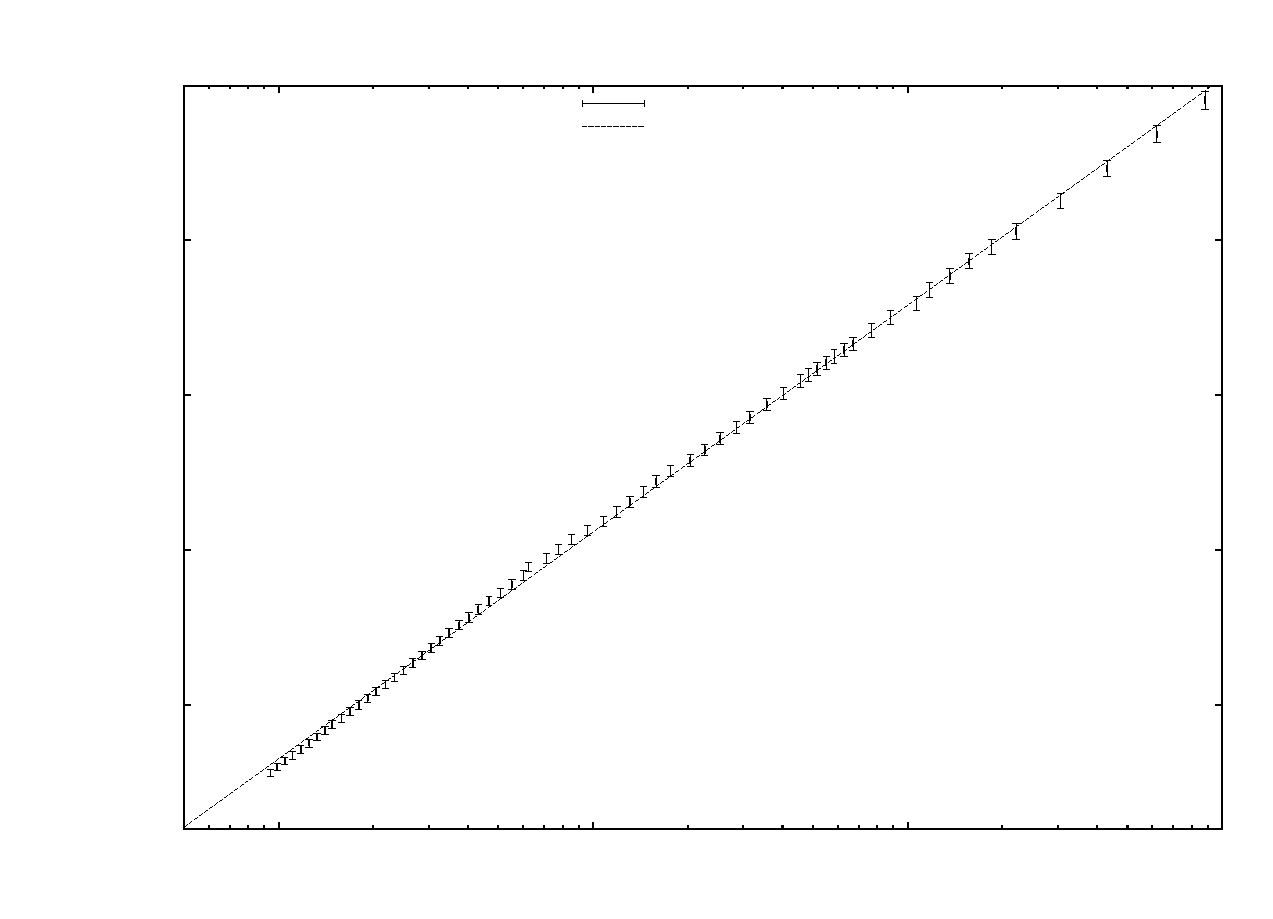
\includegraphics{graf2}}%
    \gplfronttext
  \end{picture}%
\endgroup

}
\label{g2}
\end{figure}

\begin{figure}
\scalebox{0.7}{
\input{graf3.tex}
}
\label{g3}
\end{figure}

\section{Diskuze}
Díky odečtu z multimetrů za pomoci počítače naměřené hodnoty reálně odpovídají stejným časům, což především napomohlo 
při měření odporu za nízkých teplot, který se rychle měnil. Mohl jsem naměřit více hodnot, ale podle mě by hustší data 
přesnosti fitů příliš nepomohla. Trochu menší chyby šlo dosáhnout u nízkých odporů, kdy program nepodporoval nejnižší rozsah. 
Zlepšení by však bylo nevýrazné. Slabinou měření se ukázal regulátor proudu na zdroji napětí při jeho užití na žhavení. 
Sice díky slabému výkonu nedošlo k narušení tepelné rovnováhy, ale měření se stalo velmi zdlouhavým a v daném čase jsem nedosáhl 
vyšších teplot.

\section{Závěr}
\noindent
Proměřil jsem VA charakteristiku termistoru, která je na obrázku \ref{g1}. \\
Změřil jsem teplotní závislost termistoru an teplotě. Hodnoty jsou v tabulce \ref{TTR}. \\
Graficky jsem znázornil závislost logaritmu odporu termistoru na převrácené teplotě teploty a z fitu určil hodnoty 
\begin{eqnarray}
B=(3140\pm 10) \mbox{K},\\
R_\infty=(0.0138\pm 0.0005) \mbox{k}\Omega,\\
\Delta U=(8670\pm30)\cdot10^{-23} \mbox{J},\\
\alpha=(-0.0355\pm0.0003)\mbox{K}^{-1}.
\end{eqnarray}
Stanovil jsem teplotu termistoru v maximu VA charakteristiky
\begin{eqnarray}
T_m=284.6\pm0.2 \mbox{K}
\end{eqnarray}
a tepelný odpor termistoru
\begin{eqnarray}
K=(2050\pm10)\mbox{KW}^{-1}.
\end{eqnarray}

\begin{thebibliography}{5}
	\bibitem{text} \textbf{Studijní text na praktikum II} \\http://physics.mff.cuni.cz/vyuka/zfp/txt\_209.pdf (12. 10. 2011)
    \bibitem{chyba} \emph{J. Englich}: \textbf{Zpracování výsldků fyzikálních měření} \\ LS 1999/2000
\end{thebibliography}


\end{document}
